\documentclass{article}

\usepackage[preprint]{neurips_2026}

\usepackage[utf8]{inputenc}
\usepackage[T1]{fontenc}
\usepackage[hidelinks]{hyperref}
\usepackage{url}
\usepackage{booktabs}
\usepackage{amsmath}
\usepackage{amssymb}
\usepackage{graphicx}
\usepackage{microtype}
\usepackage{xcolor}

\title{The Instrument Moves: Unrecorded Serving Changes in Agent Benchmarks}

\author{Jingyuan Yi\\ Independent Researcher\\ \texttt{jingyuay@alumni.cmu.edu}}

\begin{document}
\maketitle

\begin{abstract}
Agent benchmarks are instruments for measuring capability, and their outputs are
read as measurements. We pinned every control a mobile-agent benchmark exposes
(model identifier, serving provider, quantization, temperature, seed, image
digest, task-set commit, one fresh container per repetition, serial execution)
and ran ten repetitions. Three things followed. First,
\texttt{temperature{=}0} with a fixed seed did not produce determinism on either
endpoint we tried. Our first check said otherwise: a short prompt came back
byte-identical twice, on an endpoint that turned out not to be deterministic.
Second, ten and a half hours in, the pinned endpoint's behaviour changed. Ten
tasks got worse and none got better. Median completion tokens per action fell
by a fifth at a single round boundary and stayed there. We observed the
endpoint's behaviour, not its configuration: the shift was sudden, specific to
that endpoint, absent from a control, and invisible to every field a
leaderboard records. Third, for this agent, this endpoint and this reweighted
task sample, two single-run scores need to differ by roughly eight points
before the gap exceeds what repetition alone produces. The token signal flagged
the shift at the round level; the score did not. The signal costs one integer
per request to log. We argue that an evaluation harness should be treated as a
verification system rather than a score generator. Data, analysis code and
figure scripts: \url{https://github.com/Universeyi/instrument-moves}.
\end{abstract}

\section{Introduction}

Leaderboards for agent benchmarks are read as measurements. The gap between
adjacent entries is cited as evidence that one system is better than another,
and differences of two or three points routinely carry that weight. On the
board we study, 37 of 40 entries are the result of a single run, and no entry
reports an interval.

A benchmark that drives a real operating system through a real user interface
against real network services will have run-to-run variance. That is the price
of not being a static test set, and it is a price worth paying: the alternative
measures something much less like deployment. What has been missing is a
number for it, and a way to tell when the number has changed.

We pinned every control the tooling of
MobileWorld~\citep{kong2026mobileworld} exposes and ran ten repetitions over 29
GUI-only tasks, 290 runs in total. We set out to measure a noise floor. We
found something larger: the configuration was not, in the event, fixed, and
nothing in the tooling or the reporting format would have told us.

\paragraph{The claim.} A benchmark is an instrument for measuring agent
capability. This instrument moves while nobody is recording, and current
reporting practice contains no mechanism that would reveal it.

\paragraph{Contributions.}
\begin{itemize}\itemsep2pt
\item \textbf{A methodological error in determinism checks.} Identical requests
  at \texttt{temperature{=}0} with a fixed seed returned different completions
  on both endpoints we tested, though both advertise seed support. An earlier
  check of ours with a short prompt returned byte-identical output twice and
  looked like proof of the opposite. Under greedy decoding a thirty-token answer
  comes back byte-identical almost regardless of the endpoint; determinism has
  to be probed at the output length the real workload produces.
\item \textbf{A documented mid-run serving change, with a detector.} Between
  repetition 3 and 4, with every flag unchanged, ten tasks got worse and none
  got better ($p = 0.002$), and median completion tokens per action fell 20.1\%
  in one step. We give five independent lines of evidence and the cheap signal
  that exposes it.
\item \textbf{A noise floor for this configuration, and what it implies.}
  Within one serving configuration, two single runs need to differ by
  8.15 points before the gap exceeds what repetition alone produces. The figure
  is a property of a resampling model fitted to one agent, one endpoint and one
  reweighted task sample, not a constant of the benchmark.
\item \textbf{Findings that need no compute.} Eight properties of the public
  repository, each with where to look, that bear on whether two entries
  are comparable at all. A reader can check each one without trusting any
  measurement of ours.
\end{itemize}

A benchmark that reports only a scalar score is a measuring device with no
self-check: it cannot distinguish a system that improved from an instrument
that moved, and neither can the metadata recorded beside it. Treating the
harness as a verification system --- recording the signals a failure would show
up in, not only the number --- is what made Section~\ref{sec:endpoint} visible
at all, at a cost of one integer per request.

The first three compose into one argument rather than three results, and the
fourth asks for no trust at all. Determinism controls are why one must pin the
endpoint; the endpoint change is why pinning is not enough and why nothing would
have told us; the noise floor prices the consequence.

\section{Setup: what was pinned}
\label{sec:setup}

Table~\ref{tab:setup} is the configuration. Everything in it is a flag we could
set. This paper is about what remained free anyway.

\begin{table}[t]
\centering\small
\caption{The pinned configuration. Nothing under the benchmark was modified;
the custom agent is supplied through the harness's existing
\texttt{--agent-type} hook, so reproducing this requires no fork.}
\label{tab:setup}
\begin{tabular}{ll}
\toprule
model & \texttt{moonshotai/kimi-k2.5} via an inference router \\
serving endpoint & provider pinned, quantization \texttt{int4},
                   \texttt{allow\_fallbacks: false} \\
sampling & \texttt{temperature=0}, \texttt{seed=42},
           \texttt{max\_tokens=2048} (the agent default) \\
container image & tag \texttt{v1.4}; the full digest is recorded on every row and given in Appendix~\ref{app:provenance} \\
task-set commit & \texttt{83e7b8fc} \\
execution & \texttt{--max-concurrency 1}, no task shuffling,
            one fresh container per repetition round \\
round budget & \texttt{--max-round 50}, \texttt{--auto-retry 10} \\
tasks & 29 GUI-only, stratified from the published trajectory bundles \\
pass threshold & \texttt{score > 0.99}, the benchmark's own \\
\bottomrule
\end{tabular}
\end{table}

\paragraph{Task selection, and why it is skewed on purpose.} The 29 tasks are
drawn from the benchmark's own published per-model trajectories: 10 that the
published runs disagree on, 9 that all of them pass, and 10 that all of them
fail.\footnote{%
The groups were assigned from the 15 of the 18 published bundles whose result files our parser read;
the other three record results in formats it did not recognise. Read in full, five of the 29 tasks would
carry a different group label: four \emph{all-pass} tasks (\texttt{AcceptMeetingTask},
\texttt{CheckEventTimeTask}, \texttt{GoogleMapsAlibabaSouthNeighborTask}, \texttt{TakeSelfieTask})
each have one or two failing runs among the extra three, and one \emph{all-fail} task
(\texttt{SMSManagement}) has one passing run. The selection and every measurement are unchanged; only the
label describing the published runs differs.} The disagreed-on group is where within-configuration instability is most
likely to appear; the other two are controls, and a setup that produced flips
everywhere would be measuring something other than the benchmark. Because the
set is deliberately unrepresentative, its absolute score level is not
comparable to a leaderboard number. Only widths are, and only after the
reweighting in Section~\ref{sec:noise}.

\paragraph{Records kept per run.} The harness alone records none of the fields
above; what our orchestrator adds, and how every figure traces back to the raw
records, is catalogued in Appendix~\ref{app:provenance}. The raw records, the
endpoint probes behind Section~\ref{sec:determinism} and evidence strands 4 and
5 of Section~\ref{sec:endpoint}, the analysis code with its derived data files,
and the figure scripts are released together at \url{https://github.com/Universeyi/instrument-moves}.

\section{\texttt{temperature=0} is not determinism}
\label{sec:determinism}

Holding the model still is the first thing a careful experimenter does, and the
obvious lever is greedy decoding with a fixed seed. It does not work, and the
convenient way of checking that it works reports that it does.

We sent the same prompt three times to each of two endpoints serving the same
model, at \texttt{temperature=0} with \texttt{seed=42}. Both endpoints
advertise \texttt{seed} support in the router's capability listing. All three
completions differed on both endpoints, with lengths varying roughly twofold
(1571 / 2812 / 1427 tokens on one, 2963 / 1448 / 1494 on the other).

\paragraph{The trap.} An earlier version of this check used the prompt
\emph{``Reply with exactly: OK''}. It returned byte-identical output twice, and
we recorded that the endpoint was deterministic. It is not. Under greedy decoding a thirty-token answer will almost always come back
byte-identical, because the divergence that matters accumulates over long
generations; the check therefore cannot distinguish a deterministic endpoint
from a non-deterministic one. \textbf{Determinism has to be probed at the
output length the real workload produces.} We report this because the cheap
check is the one a practitioner will reach for, and it gives the wrong answer
in the reassuring direction.

\paragraph{Relation to known results.} That low-precision inference is
non-reproducible across serving configurations is established:
\citet{yuan2025nondeterminism} trace it to the non-associativity of
floating-point arithmetic and show that batch size, GPU count and GPU version
alone move accuracy by up to nine points under \texttt{bfloat16} greedy
decoding. Our contribution here is not the phenomenon. It is that the
phenomenon is invisible to the standard sanity check, and that a hosted
endpoint gives a practitioner no way to hold those variables fixed --- batch
composition is a property of other customers' traffic.

\paragraph{Consequence for the rest of this paper.} Because sampling cannot be
held still, we do not claim any decomposition of variance into
``environment'' and ``model'' parts. What Section~\ref{sec:noise} reports is
the total variation that survives every control available to a careful
experimenter, which is the quantity a reader comparing two leaderboard entries
actually faces.

\section{The endpoint moved}
\label{sec:endpoint}

Ten and a half hours into a thirty-three hour run, between repetition round 3
(which ended 2026-08-26 06:47 UTC) and round 4 (which began 06:49 UTC), the
results changed character. Nothing changed on our side: same image
digest, same task-set commit, same model identifier, same pinned provider and
quantization, same temperature and seed, same code.

\begin{figure}[t]
\centering
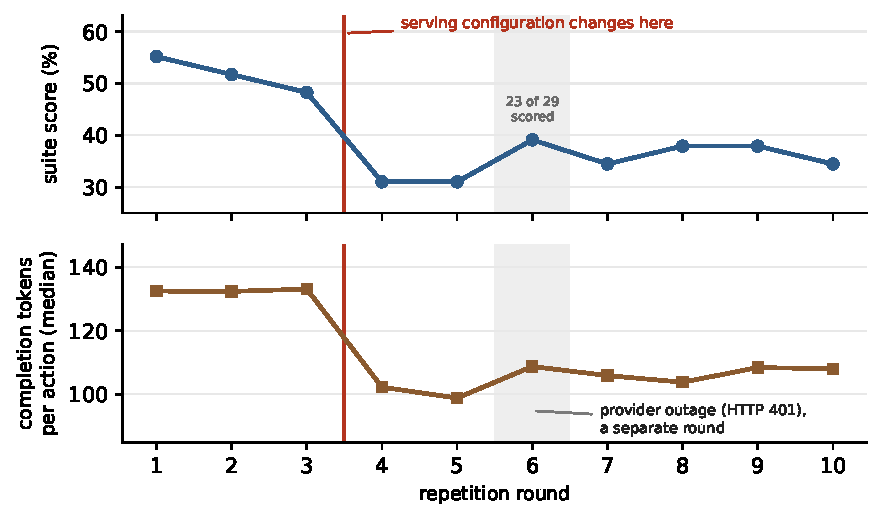
\includegraphics[width=0.80\textwidth]{figures/fig_regime.pdf}
\caption{Suite score and reasoning volume per repetition round, on a shared
axis. Both step at the same place, between rounds 3 and 4 (red line), and both
hold at the new level for the remaining seven rounds. The provider outage
(shaded, round 6) is a separate event at a different round; the step is not the
outage. Round 6 scored 23 of 29 tasks and is annotated accordingly. Two stacked
panels rather than one plot with two vertical axes, so that no choice of scale
can be doing the work.}
\label{fig:regime}
\end{figure}

\subsection{Five checks on the same trajectories, corroborated outside them}

\paragraph{1. Every task that moved, moved the same way.} Ten tasks changed
pass rate across the boundary; all ten got worse, none improved, nineteen were
unchanged. Figure~\ref{fig:dumbbell} shows all ten arrows pointing the same
way, which repetition noise alone would rarely produce: an exact sign test on the
ten gives $p = 0.002$. We read that as an indication of how one-sided the split
is rather than as a hypothesis test at face value, since tasks within a round
share a container, the backend services and an execution order, and so are not
strictly independent.

\begin{figure}[t]
\centering
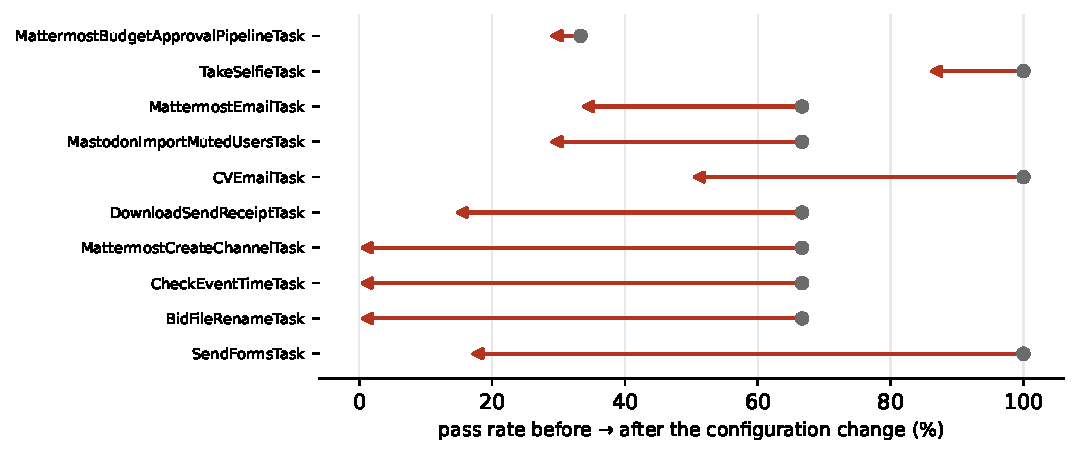
\includegraphics[width=0.86\textwidth]{figures/fig_dumbbell.pdf}
\caption{Per-task pass rate before and after the boundary, one arrow per task
that moved. Ten tasks moved and all ten moved the same way: 10 worse, 0 better,
19 unchanged (exact sign test $p = 0.002$, read as an indication of how
one-sided the split is; tasks within a round are not strictly independent).}
\label{fig:dumbbell}
\end{figure}

\paragraph{2. Reasoning volume stepped, and did not drift.} Median completion
tokens per action --- one step is one model request, and the output is almost
entirely reasoning --- were 132.5, 132.4, 133.1 in rounds 1--3, within 0.55\%
of each other, and 102.2, 98.8, 108.7, 105.9, 103.8, 108.4, 108.0 in rounds
4--10, spanning 98.8--108.7, about $\pm$4.8\% around the regime midpoint.
Between the two regimes the median fell 20.1\%.

\paragraph{3. Faster and worse at the same time.} Comparing rounds 1--3 with
rounds 4--10 throughout (round 6 in, its six zero-step no-verdict runs out):
mean time per step fell from 16.0\,s to 13.7\,s while
quality fell. Degrading hardware or a congested network makes an endpoint
slower, not quicker. Generating less reasoning per call explains both
directions at once, and it explains the third-order effects too: mean steps per
run rose from 28.7 to 30.6 and the share of runs stopped by the 50-step budget
rose from 31\% to 45\%.

\paragraph{Time of day does not explain it.} Co-tenant traffic changes batch
composition --- the mechanism \citet{yuan2025nondeterminism} identify --- so a
diurnal effect is a live alternative. Our own schedule rules it out: rounds
9--10 ran 22:21--04:51 UTC, inside the same overnight window as rounds 1--3
(20:10--06:47 UTC), and stayed at the post-shift level. A daily cycle cannot
produce a step that survives a return to the original hours.

\paragraph{4 and 5. Corroborated outside the harness, with a control.} The
determinism probe of Section~\ref{sec:determinism}, unchanged, sent to the
pinned endpoint on two consecutive days: on the first day the three completions
ranged from 1427 to 2812 tokens (sample SD 761), and on the second day they
came back nearly identical (1344, 1292, 1292; sample SD 30). The same probe
against a second provider serving the same model gave 2963, 1448, 1494 on the
first day and 1938, 1672, 2427 on the second, varying on both days. Each cell
is three requests, so we describe rather than test, and we report sample SD
throughout. The probe locates the change to a day; the round boundary comes
from the harness's internal timing. The harness is not involved in either
measurement, and the change in behaviour was specific to the endpoint we had
pinned rather than to the model, the prompt or our tooling.

\paragraph{What we observed, and what we infer.} We observed an endpoint's
behaviour, not its configuration. A serving-side change is the only explanation
we know of that accounts for all of it at once, but we cannot rule out
explanations we have not thought of, and nothing below depends on the cause.

\subsection{Why this is the finding}

Every one of these controls exists and we set it. There is no flag that pins
how a provider serves the model, because serving behaviour is not part of the
API contract; it is an operational property of somebody else's fleet. And there
is no field in any leaderboard entry, on this board or the others we looked at,
that records which configuration produced the number.

This is not a property of the benchmark we happened to use. Any evaluation
built on hosted inference is exposed to this gap between what the submitter
controls and what determines the number, and the more an agent's behaviour
depends on long reasoning chains, the more exposed it is. We observed one such
change in ten repetitions; we have no measurement of how often they happen,
and nothing here should be read as a claim that they are routine.

\paragraph{A cheap side signal, offered with its limits.} The quantity that
made this visible is completion tokens per action. The harness records
\texttt{total\_tokens}, which is 98.5\% prompt in this workload and moved by
8\% across the change: not enough to notice. Completion tokens per action moved
20.1\% in one step, and a per-round check of the kind our sentinel uses fires
on it at the boundary round while a score test at the same granularity does
not. We call this a side signal, not a detector: it has
worked once, after the fact. A sentinel probe logging fixed requests to 14
endpoints over three weeks raised five length alarms in 328 endpoint-days, none
on two consecutive days; day-shuffled calibration puts the false-alarm rate at
0.06\%. The sentinel measures the output length of fixed requests, a close
relative of tokens per action rather than the same quantity, and a quiet period
calibrates false alarms, not sensitivity. Recording the signal cost nothing
and we had to recover it from raw trajectories after the fact. We recommend
logging it by default (Section~\ref{sec:recs}).

\section{The resulting noise floor}
\label{sec:noise}

Seven repetitions fall inside the later serving configuration. They scored
31.0, 31.0, 39.1, 34.5, 37.9, 37.9 and 34.5\%. \emph{Every headline figure
below is computed on the six rounds that exclude round 6, for the reason given
after Table~\ref{tab:loo}; seven-round values are given alongside so the
difference is always visible.} Seven of 29 tasks did not return the
same verdict every time (eight over all seven rounds), and the controls behave
as they should: 0 of 10 flips among tasks all published runs fail, 1 of 9 among
tasks all published runs pass, and 6 of 10 among the disagreed-on group.

\paragraph{The headline is not the range.} A best-minus-worst spread is an
order statistic: it cannot grow when a repetition is removed, it grows on
average with the number of repetitions, and a seven-round spread and a
six-round spread are therefore not comparable quantities. Our own sensitivity
check forced this correction. Table~\ref{tab:loo} recomputes everything with
each round dropped in turn: the spread is unmoved by dropping any round except
the one holding the maximum, while the minimum detectable difference varies
across all seven variants within a narrow band. Throughout, the
\emph{detectable difference at 95\%} is $1.96\sqrt{2}\,\sigma$, with $\sigma$
the resampled single-run standard deviation at the reweighted 117-task scale;
interval widths beside it are empirical 2.5--97.5\% spans of the same
distribution, hence not exact multiples (Appendix~\ref{app:intervals}).

\begin{table}[t]
\centering\small
\caption{Leave-one-round-out. Every figure recomputed from scratch on what
remains. The range responds only to removing the maximum; the detectable
difference is stable at 8.02--9.01 points and the comparison against published
entries never changes.}
\label{tab:loo}
\begin{tabular}{lccccccc}
\toprule
round dropped & 4 & 5 & \textbf{6} & 7 & 8 & 9 & 10 \\
\midrule
best $-$ worst (pp) & 8.10 & 8.10 & \textbf{6.90} & 8.10 & 8.10 & 8.10 & 8.10 \\
detectable difference (pp) & 9.00 & 8.52 & \textbf{8.15} & 8.42 & 8.02 & 8.76 & 9.01 \\
adjacent gaps within noise & 16/17 & 16/17 & 16/17 & 16/17 & 16/17 & 16/17 & 16/17 \\
\bottomrule
\end{tabular}
\end{table}

\paragraph{Round 6, and why the conservative number is the headline.} Round 6
contains the only infrastructure incident in the run: the provider returned
HTTP 401 for about an hour, 68 of the 95 silent restarts in this regime fall in it (110 across all ten rounds), and
all six runs that produced no verdict are in it. It is also the highest-scoring
round of the regime, on a reduced denominator of 23 tasks. We therefore report
the figures \emph{without} it as the headline, with the seven-round values
alongside:\footnote{The two scales move in \emph{opposite} directions when round
6 is removed: at the 29-task scale $\sigma$ rises from 5.87 to 5.92\,pp, at the
reweighted 117-task scale it falls from 3.13 to 2.94\,pp. They are computed
differently, and Appendix~\ref{app:sensitivity} traces the mechanism; the
detectable difference derives from the second scale. We report both because
reporting only the one that suits the argument is precisely the failure this
paper is about.}

\begin{center}\small
\begin{tabular}{lcc}
\toprule
 & 6 rounds (round 6 removed) & 7 rounds \\
\midrule
detectable difference at 95\% & \textbf{8.15 pp} & 8.67 pp \\
95\% interval at suite scale, width & \textbf{11.11 pp} & 12.82 pp \\
tasks that flipped & 7 / 29 & 8 / 29 \\
\bottomrule
\end{tabular}
\end{center}

\textbf{Removing the incident moves the result against us, and we report it
anyway.} The threshold falls from 8.67 to 8.15 points, which is a stricter bar:
the number of published pairs separated by less than it drops from 39 to 35.
We report the lower figure because it is the one measured on data containing no
infrastructure incident, not because it is the more favourable one.

Two things are worth stating precisely rather than glossing. First, the single
task that stops flipping, \texttt{DownloadSendReceiptTask}, does so at 1/7
$\rightarrow$ 0/6: it lost its one passing round, not its instability. Only 4 of
29 tasks change pass rate at all, and no task flips \emph{only} when round 6 is
removed. Second, imputing the six lost runs at those tasks' own rates in the
other rounds puts round 6 at 40.2\% rather than the 39.13\% recorded --- the
outage cost that round height rather than lending it any, because the tasks it
happened to cost pass more often than average (44.4\% against 34.5\%).
Appendix~\ref{app:sensitivity} has the full comparison.



\paragraph{Carrying it to the full suite.} The 29 tasks are deliberately
skewed, so their level means nothing on its own. Reweighting the three groups
to their true sizes in the 117-task GUI-only suite (98 disagreed-on, 9
always-passed, 10 always-failed) gives a width that is comparable to a
leaderboard number. Stated conditionally, because it is:
\emph{if the 88 disagreed-on tasks we did not measure behave like the 10 we
did}, a single run of the full suite falls within a 95\% interval about
11.1 points wide.

\paragraph{What this means for reading a leaderboard.} Under the resampling model above, and for this agent on this endpoint, two
single runs need to differ by 8.15 points before the gap exceeds what
repetition alone produces; to detect a real difference reliably rather than merely to notice it,
the gap must be larger still. Of the 17 adjacent pairs among the 18 published GUI-only entries, 16 are
separated by less than that, as are 35 of the 153 pairs overall (39 at the
seven-round threshold of 8.67). We state this as an indication of scale and not as a re-scoring: the
threshold was measured for one model on 29 tasks and is being applied to
entries produced by other agents and other models. The appropriate reading of a
gap below the threshold is that it \emph{warrants a second run before
citation}, not that the two systems are equal.

\paragraph{Are the flips scoring errors rather than variance?} It is the
obvious alternative explanation, and we checked it: we inspected the five
most suspicious of 111 ranked runs against the task definitions and found no
verifier defect --- every one was a genuine agent failure. Appendix~\ref{app:checker}
reports that negative result and why we had every incentive to find the
opposite.

\section{What is already true without running anything}
\label{sec:zerocompute}

Everything above rests on measurements a reader has to take on trust until the
data is inspected. This section does not. Table~\ref{tab:zero} lists eight
properties of the public repository at the pinned commit, each checkable in a
few minutes, each bearing on whether two entries on one leaderboard are
comparable. We re-verified all eight against commit \texttt{83e7b8fc} while
drafting.

\begin{table}[t]
\centering\footnotesize
\caption{Checkable without running the benchmark. Line numbers are at commit
\texttt{83e7b8fc}; step-count statistics are computed from the benchmark's own
published per-model trajectories.}
\label{tab:zero}
\begin{tabular}{p{0.28\textwidth}p{0.25\textwidth}p{0.39\textwidth}}
\toprule
\textbf{Verifiable fact} & \textbf{Where} & \textbf{Consequence for comparability} \\
\midrule
For model ids containing \texttt{claude}, \texttt{max\_tokens} is set to 64000;
every other model uses the agent default of 2048.
& \texttt{agents/base.py:97--99}
& Entries on one board run under generation budgets differing by a factor of
31, and no field records it. Room to reason is what
Section~\ref{sec:endpoint} shows moving the score; we claim the structural
difference only, no entry's counterfactual. \\
\addlinespace
Of 2562 published (model, task) runs with a step count, 525 (20.5\%) sit at
exactly 50 steps, against 18, 10, 20 and 2 at 48, 49, 51 and 52. 490 of the 525
(93.3\%) scored 0 and 35 passed.\footnotemark
& published trajectories
& One run in five ends at a budget rather than at a task outcome; the record
shows a zero, not which event occurred. \\
\addlinespace
All 30 runs above 50 steps belong to a single entry, which has no runs at
exactly 50; the other 17 entries have runs at 50 and none above.
& published trajectories
& At least two different round budgets produced the published board, and no
entry records which applied. Under one 50-step budget the region above 50
would be empty; it is not --- a different budget, not a lucky escape. \\
\addlinespace
For model ids containing \texttt{claude}, \texttt{temperature} is deleted from
the request.
& \texttt{agents/base.py:97--99}
& Those entries ran at the provider's default sampling, not at the value the
harness otherwise sets. \\
\addlinespace
Verifier corrections \texttt{8ae5064}, \texttt{c33e340}, \texttt{32ed916} and
\texttt{702e904} postdate existing entries.
& repository history
& Entries from different dates were scored by different verifier versions, and
no entry records which. \\
\addlinespace
For model ids containing \texttt{kimi-k}, \texttt{extra\_body} is assigned
rather than merged, discarding whatever the caller supplied.
& \texttt{agents/base.py:105--106}
& Provider and quantization pinning supplied by a caller never reaches the API.
This is how we found it: requests we believed pinned were served by three
different providers. \\
\addlinespace
The cleanup path matches containers against a hardcoded \texttt{:latest} image.
& \texttt{runtime/utils/}\allowbreak\texttt{models.py:28}
& With a pinned image tag, \texttt{mw env rm --all} reports success while
containers keep running. \\
\addlinespace
The emulator is started with \texttt{-no-snapshot}.
& \texttt{docker/}\allowbreak\texttt{start\_emulator.sh:5}
& The documented guarantee of identical initial state via AVD snapshots is not
what executes. \\
\bottomrule
\end{tabular}
\end{table}
\footnotetext{%
The version submitted for review reported 90 of the runs at the cap as carrying no score at all. Three of
the 18 bundles record results in formats our first parser did not read; read in full, every run at the cap
has a score, and the 90 split into 83 zeros and 7 passes.}

None of this requires trusting a measurement of ours. It requires reading the
repository. One nuance is empirical rather than read from code: the 30 runs
above the cap sit at 51--54, and a plausible innocent cause is a custom agent
setting its own bound --- whichever it is, the board does not say.

\section{Recommendations}
\label{sec:recs}

These are addressed to benchmark maintainers and to anyone reporting agent
evaluations, ourselves included. They are cheap, and most of them are fields
rather than experiments.

\begin{enumerate}\itemsep2pt
\item \textbf{Record the serving endpoint, not just the model identifier.}
  Provider and quantization at minimum. Two entries carrying the same model id
  today can be different weights on different hardware, and a reader has no way
  to tell. This is the single highest-value change here, and it is one column.
\item \textbf{Record image digest, task-set commit and run date.} Digest rather
  than tag: a tag moves. The run date is what lets a reader notice that two
  entries are separated by an unannounced change in endpoint behaviour.
\item \textbf{Report the number of runs, and a range when there is more than
  one.} Three runs with a minimum and maximum costs three times the compute and
  removes most of the ambiguity. Where a board already stores a run count,
  surfacing it in the rendered table is free.
\item \textbf{State a minimum meaningful gap in the leaderboard
  documentation.} The same-system difference threshold of
  Section~\ref{sec:noise} is one way to compute one; resampling whole rounds
  puts it between 5.18 and 8.53 points. Differences below that range between
  single runs are not resolvable. Saying so protects submitters as much as
  readers: it removes the incentive to claim a lead that a re-run would
  erase.
\item \textbf{Log completion tokens per action.} It is the cheapest available
  witness to an endpoint changing underneath a run. Aggregate token counts are
  dominated by the prompt and will not show it.
\item \textbf{Distinguish budget exhaustion from task failure in the recorded
  outcome.} A run stopped at the round cap and a run that did the wrong thing
  are different events; one in five published runs is the former.
\item \textbf{Three small fixes we can offer upstream}, each independent of
  everything above: merge rather than assign caller-supplied request options;
  guard the response-content accessor against a \texttt{None} body, which a
  reasoning model returns when it exhausts its budget mid-thought; and match
  container cleanup against the configured image rather than a hardcoded tag.
\end{enumerate}

There is a stronger conclusion available, and our data supports it: if a
serving configuration is not part of an API contract, then an evaluation built
on hosted inference is not reproducible in principle, only in practice and only
until the provider changes something. The strict remedy is to self-host and
freeze the weights. We are not proposing that everyone do so --- for most
groups the cost is prohibitive and the hosted endpoint is the thing they
actually deploy against --- but a field that cites two-point differences should
be explicit that it has chosen convenience over reproducibility, rather than
assuming it has both.

None of this makes a benchmark deterministic, and none of it should. The
purpose is narrower: to let a reader of a leaderboard tell the difference
between a system that improved and an instrument that moved.

\section{Limitations}

\textbf{One agent, one model, one endpoint.} Instability is very likely
model-dependent: a model that is decisive on a task will flip less than one
that is borderline on it. The threshold we report should be read as an order of
magnitude for this class of benchmark, not as a constant to be applied to other
entries as though it were measured on them.

\textbf{Seven repetitions over 29 tasks.} Per-task rates are correspondingly
imprecise --- a task passing 3 of 6 times has a 95\% interval of roughly
19--81\%. The suite-level figures are much better determined than the per-task
ones, and we lean on the former.

\textbf{The task set is deliberately skewed} toward tasks that published runs
disagree on. Its score level is not comparable to a leaderboard number; only
the width is, and only after reweighting, and that reweighting assumes the 88
disagreed-on tasks we did not run behave like the 10 we did.

\textbf{GUI-only.} The user-interaction and MCP suites were not run. The former
puts a second language model inside the loop and would plausibly be noisier,
not less.

\textbf{The harness absorbs part of what we set out to measure.} Its internal
retry fired 110 times across all ten rounds (95 of them within the seven rounds
of the headline configuration), silently, and those restarts are instability
that never reached a score. Our figures are therefore a floor.

\textbf{Environment version.} We ran a container image newer than the one most
published entries used, because the older tag carries a defect the maintainers
had already fixed and injecting a known bug into a variance measurement would
measure the wrong thing. The quantization also differs from the reference
entry's. Both are recorded per run.

\textbf{The serving change is documented, not explained.} We can show when it
happened, that it was specific to one endpoint, and what it did to the output.
We cannot see inside somebody else's fleet, and we do not speculate about the
cause.

We would rather see this measured better than see it left unmeasured. The raw
per-run records, the analysis code and the figure scripts are released, and the
figures in this paper regenerate from a single command. If the noise floor of
an evaluation instrument is worth knowing --- and we think a field that cites
two-point differences should want to know it --- then it is worth publishing
alongside the scores, by whoever is best placed to measure it.

\section{Related work}

\paragraph{Mobile and GUI agent benchmarks.} Interactive Android environments
with programmatic reward signals were established by
AndroidWorld~\citep{rawles2025androidworld}, which supplies tasks across real
applications on a live emulator rather than a static test set. MobileWorld
\citep{kong2026mobileworld}, the benchmark studied here, extends that setting
with agent--user interaction and MCP-augmented tasks and publishes a leaderboard
together with per-model trajectories. Our use of it is not adversarial: the
published trajectories are what made the zero-compute analysis of
Section~\ref{sec:zerocompute} possible at all, and few benchmarks release
enough for an outsider to do it.

\paragraph{Nondeterminism in language model inference.}
\citet{yuan2025nondeterminism} establish that low-precision inference is not
reproducible across serving configurations, tracing it to the non-associativity
of floating-point arithmetic and showing that batch size, GPU count and GPU
version alone can move accuracy by several points under greedy decoding. That
work explains the mechanism behind our Section~\ref{sec:determinism} and,
plausibly, behind Section~\ref{sec:endpoint}. The difference in setting matters:
their variables are controllable by whoever owns the hardware, whereas a
practitioner calling a hosted endpoint controls none of them and cannot observe
them either --- batch composition is a function of other customers' traffic.

\paragraph{Drift in hosted model services.} That a commercial model endpoint
changes behaviour over time is established. \citet{chen2024chatgpt} evaluated
the March and June 2023 releases of two hosted models across several task
families and found large swings --- identification of prime versus composite
numbers fell from 84\% to 51\% accuracy on one of them --- and argued for
continuous monitoring. The same group had earlier framed the general problem of
detecting shifts in machine learning APIs efficiently~\citep{chen2021apishifts}.

Our setting is narrower and, we think, harder to defend against. That work
compares \emph{labelled versions} of a service \emph{months apart}, and detects
the change by periodically re-running a whole evaluation suite. What we record
happened inside a single model identifier, at one provider, at one
quantization, within \emph{a single half-day}, with no version change announced or
announceable --- and it was caught not by re-running an evaluation but by a
cheap side signal, completion tokens per action, that costs one integer per
request to log. The first result tells a practitioner that a service will
change. The second tells them it can change \emph{during their experiment},
while every control they know about is still set, and that the standard check
will not show it.

\paragraph{Flaky tests.} Software engineering has a mature literature on tests
that pass and fail without a code change, including how practitioners
experience and manage them~\citep{gruber2022flakiness}. The analogy is close
and the vocabulary is useful, but the disanalogy is the point of this paper: a
flaky test is understood as a defect to be fixed, whereas run-to-run variance
in an environment-driven agent benchmark is a property of the measurement that
should be quantified and reported rather than eliminated. The software
engineering framing also assumes the system under test is the thing that
varies. Here the harness, the environment and the serving endpoint all vary,
and only one of them is the object of measurement.

\paragraph{Statistical reporting for evaluations.}
\citet{miller2024errorbars} sets out error-bar methodology for LLM evals,
\citet{bowyer2025clt} caution that CLT intervals understate uncertainty at
task counts like ours, and $\tau$-bench~\citep{yao2025taubench} reports
run-to-run inconsistency as a metric, pass\textasciicircum{}$k$. All three
hold the thing measured stationary while it is measured.
Section~\ref{sec:noise} is what their machinery yields here;
Section~\ref{sec:endpoint} is the case none of them models --- the instrument
moving mid-experiment.

\paragraph{Positioning.} These lines of work measure model or agent capability,
or the reliability of a test suite. This paper measures the instrument: how far
a benchmark's own output moves when its input is held as fixed as the available
controls allow, and what a reader would need recorded in order to notice when
it moves for reasons that have nothing to do with the agent.


\bibliographystyle{plainnat}
\bibliography{refs}

\appendix
\section{Per-task results}
\label{app:pertask}
All 29 tasks over the six repetitions of the headline basis, ordered by flip
rate. \textbf{The \emph{group} column describes the published runs' behaviour,
not ours}: it records whether the benchmark's own published trajectories all
passed a task, all failed it, or disagreed on it (Section~\ref{sec:setup}), and
it is how the task set was stratified. A task can therefore be listed as
\emph{all-pass} and still have failed in every one of our repetitions.\footnote{%
Four tasks here score 0/6 despite having passed in two of the three rounds that
preceded the shift in behaviour of Section~\ref{sec:endpoint}:
\texttt{BidFileRenameTask}, \texttt{CheckEventTimeTask},
\texttt{DownloadSendReceiptTask} and \texttt{MattermostCreateChannelTask} (see
Figure~\ref{fig:dumbbell}). The headline basis lies entirely after that change,
so these rows are a consequence of it rather than an anomaly. The remaining
zero-scoring tasks are ones the published runs also fail.} Flip rate is the share of trial pairs that disagree,
$k(n-k)/\binom{n}{2}$; its maximum is below 1 and depends on $n$, reaching
0.600 at $n=6$. Wilson intervals are wide at this sample size, which is why the
suite-level figures rather than the per-task ones carry the argument in
Section~\ref{sec:noise}.

\begin{center}\scriptsize
\begin{tabular}{llccccc}
\toprule
task & group & passed & pass rate & Wilson 95\% & flip rate & steps (median) \\
\midrule
\texttt{CVEmailTask} & disagreed & 3/6 & 50\% & 19--81\% & 0.600 & 11 \\
\texttt{ScheduleLunchViaSmsTask} & disagreed & 4/6 & 67\% & 30--90\% & 0.533 & 25 \\
\texttt{MattermostBudgetApprovalPipelineTask} & disagreed & 2/6 & 33\% & 10--70\% & 0.533 & 50 \\
\texttt{MattermostEmailTask} & disagreed & 2/6 & 33\% & 10--70\% & 0.533 & 21 \\
\texttt{TakeSelfieTask} & all-pass & 5/6 & 83\% & 44--97\% & 0.333 & 12 \\
\texttt{MastodonImportMutedUsersTask} & disagreed & 1/6 & 17\% & 3--56\% & 0.333 & 50 \\
\texttt{SendFormsTask} & disagreed & 1/6 & 17\% & 3--56\% & 0.333 & 50 \\
\texttt{AcceptMeetingTask} & all-pass & 6/6 & 100\% & 61--100\% & 0.000 & 7 \\
\texttt{ChangeWallpaperTask} & all-pass & 6/6 & 100\% & 61--100\% & 0.000 & 9 \\
\texttt{CloseFlightModeTask} & all-pass & 6/6 & 100\% & 61--100\% & 0.000 & 7 \\
\texttt{GoogleMapsAlibabaSouthNeighborTask} & all-pass & 6/6 & 100\% & 61--100\% & 0.000 & 9 \\
\texttt{MastodonChangeHeaderTask} & all-pass & 6/6 & 100\% & 61--100\% & 0.000 & 7 \\
\texttt{MastodonNewPostTask} & all-pass & 6/6 & 100\% & 61--100\% & 0.000 & 6 \\
\texttt{OpenFlightModeTask} & all-pass & 6/6 & 100\% & 61--100\% & 0.000 & 6 \\
\texttt{BidFileRenameTask} & disagreed & 0/6 & 0\% & 0--39\% & 0.000 & 50 \\
\texttt{CheckEventTimeTask} & all-pass & 0/6 & 0\% & 0--39\% & 0.000 & 20 \\
\texttt{CheckInterviewTimesTask} & all-fail & 0/6 & 0\% & 0--39\% & 0.000 & 50 \\
\texttt{DownloadSendReceiptTask} & disagreed & 0/6 & 0\% & 0--39\% & 0.000 & 34 \\
\texttt{GraduationMassEmailTask} & disagreed & 0/6 & 0\% & 0--39\% & 0.000 & 13 \\
\texttt{LocalFileManagementTask2} & all-fail & 0/6 & 0\% & 0--39\% & 0.000 & 50 \\
\texttt{MastodonCalendarMultiMemosTask} & all-fail & 0/6 & 0\% & 0--39\% & 0.000 & 50 \\
\texttt{MastodonGetServerInfoTask} & all-fail & 0/6 & 0\% & 0--39\% & 0.000 & 50 \\
\texttt{MastodonServerInfoReportTask} & all-fail & 0/6 & 0\% & 0--39\% & 0.000 & 50 \\
\texttt{MastodonShareLocationTask} & all-fail & 0/6 & 0\% & 0--39\% & 0.000 & 36 \\
\texttt{MattermostCreateChannelTask} & disagreed & 0/6 & 0\% & 0--39\% & 0.000 & 24 \\
\texttt{MattermostProjectStatusReportTask} & all-fail & 0/6 & 0\% & 0--39\% & 0.000 & 50 \\
\texttt{MattermostResourceConflictResolutionTask} & all-fail & 0/6 & 0\% & 0--39\% & 0.000 & 50 \\
\texttt{ReadQwen3PaperTask5} & all-fail & 0/6 & 0\% & 0--39\% & 0.000 & 50 \\
\texttt{SMSManagement} & all-fail & 0/6 & 0\% & 0--39\% & 0.000 & 50 \\
\bottomrule
\end{tabular}

\end{center}

\section{Tasks that never flipped}
\label{app:stable}
The 22 tasks that returned the same verdict in every repetition of the headline
basis. As in Appendix~\ref{app:pertask}, \emph{group} is the published runs'
behaviour rather than ours, which is why a row can read \emph{all-pass} and
\emph{always failed} at once. Their existence is the control: a setup that flipped everywhere would be
measuring something other than the benchmark. Note that all 10 tasks the
published runs uniformly fail are here, and 8 of the 9 they uniformly pass.

\begin{center}\scriptsize
\begin{tabular}{llcl}
\toprule
task & group & passed & outcome \\
\midrule
\texttt{CheckInterviewTimesTask} & all-fail & 0/6 & always failed \\
\texttt{LocalFileManagementTask2} & all-fail & 0/6 & always failed \\
\texttt{MastodonCalendarMultiMemosTask} & all-fail & 0/6 & always failed \\
\texttt{MastodonGetServerInfoTask} & all-fail & 0/6 & always failed \\
\texttt{MastodonServerInfoReportTask} & all-fail & 0/6 & always failed \\
\texttt{MastodonShareLocationTask} & all-fail & 0/6 & always failed \\
\texttt{MattermostProjectStatusReportTask} & all-fail & 0/6 & always failed \\
\texttt{MattermostResourceConflictResolutionTask} & all-fail & 0/6 & always failed \\
\texttt{ReadQwen3PaperTask5} & all-fail & 0/6 & always failed \\
\texttt{SMSManagement} & all-fail & 0/6 & always failed \\
\texttt{AcceptMeetingTask} & all-pass & 6/6 & always passed \\
\texttt{ChangeWallpaperTask} & all-pass & 6/6 & always passed \\
\texttt{CheckEventTimeTask} & all-pass & 0/6 & always failed \\
\texttt{CloseFlightModeTask} & all-pass & 6/6 & always passed \\
\texttt{GoogleMapsAlibabaSouthNeighborTask} & all-pass & 6/6 & always passed \\
\texttt{MastodonChangeHeaderTask} & all-pass & 6/6 & always passed \\
\texttt{MastodonNewPostTask} & all-pass & 6/6 & always passed \\
\texttt{OpenFlightModeTask} & all-pass & 6/6 & always passed \\
\texttt{BidFileRenameTask} & disagreed & 0/6 & always failed \\
\texttt{DownloadSendReceiptTask} & disagreed & 0/6 & always failed \\
\texttt{GraduationMassEmailTask} & disagreed & 0/6 & always failed \\
\texttt{MattermostCreateChannelTask} & disagreed & 0/6 & always failed \\
\bottomrule
\end{tabular}

\end{center}

\section{Three intervals that are easy to confuse}
\label{app:intervals}
We compute and report three different quantities, and conflating them is the
most likely way to misread this paper.
\begin{itemize}\itemsep2pt
\item \textbf{Re-run distribution.} Where the total would land if the same task
  set were run again. Each task's rate is drawn from a Jeffreys posterior
  before the Bernoulli draw, so that the finite number of repetitions is
  carried through rather than assumed away. This is the headline at the 29-task
  suite scale (the $\sigma$ of the footnote in Section~\ref{sec:noise}).
\item \textbf{Plug-in distribution.} The same, with each measured rate treated
  as exact. The reweighted 117-task width and the same-system difference threshold ---
  $1.96\sqrt{2}\,\sigma$ of this distribution --- derive from it. Excluding
  parameter uncertainty makes both lower bounds on the re-run width, which is
  the conservative direction for reading a gap.
\item \textbf{Estimate bootstrap.} How precisely \emph{this experiment}
  determined its own number, by resampling repetitions within each task. It
  answers a question about our precision, not about a future run.
\end{itemize}

\section{Silent restarts}
\label{app:retries}
Across the 290 runs of the arm the harness's in-task retry fired 110 times.
Every one is instability that was absorbed before it could reach a score, which
is why the variance reported in Section~\ref{sec:noise} is a floor. The
concentration is the diagnostic: a hard task is hard in every round, whereas an
incident happens in one.

\begin{center}\small
\begin{tabular}{lcccccccccc}
\toprule
round & 1 & 2 & 3 & 4 & 5 & 6 & 7 & 8 & 9 & 10 \\
silent restarts & 6 & 5 & 4 & 3 & 3 & \textbf{68} & 3 & 7 & 7 & 4 \\
\bottomrule
\end{tabular}

\end{center}

\noindent By task, counting only tasks that were restarted at least once:

\begin{center}\scriptsize
\begin{tabular}{lc}
\toprule
task & silent restarts \\
\midrule
\texttt{MastodonImportMutedUsersTask} & 13 \\
\texttt{MastodonServerInfoReportTask} & 12 \\
\texttt{MastodonShareLocationTask} & 12 \\
\texttt{AcceptMeetingTask} & 9 \\
\texttt{CVEmailTask} & 9 \\
\texttt{ChangeWallpaperTask} & 9 \\
\texttt{MattermostCreateChannelTask} & 9 \\
\texttt{MattermostEmailTask} & 9 \\
\texttt{ScheduleLunchViaSmsTask} & 9 \\
\texttt{SendFormsTask} & 9 \\
\texttt{MattermostBudgetApprovalPipelineTask} & 5 \\
\texttt{MastodonGetServerInfoTask} & 4 \\
\texttt{DownloadSendReceiptTask} & 1 \\
\bottomrule
\end{tabular}

\end{center}

\section{Method and provenance}
\label{app:provenance}
The harness records a trajectory, a screenshot per step and a free-text
verdict, but no timestamps, model parameters, image digest or task-set commit.
Our orchestrator adds those, plus the count of directories the harness leaves
behind when it silently restarts a run, and writes one \texttt{fsync}'d line
per run. The raw record (\texttt{runs.jsonl}, 314 lines covering this arm and
the preparatory smoke and calibration arms) carries a sha256 that is stamped
into the analysis file and onto every report figure; the paper's figures
regenerate from that analysis file by one seeded command, so any figure can be
traced to the records that produced it.

Every field below is recorded on each of the 290 rows and checked for
consistency across them; a row disagreeing with the others would be reported as
a violation rather than averaged over.

\begin{center}\small
\begin{tabular}{ll}
\toprule
model & \texttt{moonshotai/kimi-k2.5} \\
serving provider / quantization & \texttt{atlas-cloud} / \texttt{int4} \\
sampling & temperature \texttt{0.0}, seed \texttt{42} \\
agent & \texttt{agents/pinned\_e2e\_agent.py} \\
image & \texttt{ghcr.io/tongyi-mai/mobile\_world:v1.4} \\
image digest & \begin{tabular}[t]{@{}l@{}}\texttt{sha256:00e24a8995892af9a0e1b68bc14ce455}\\\texttt{fae288d0f1ca8cf57e84a58e40e9f19e}\end{tabular} \\
task-set commit & \texttt{83e7b8fc75ebb6c4a098254a42999db5f4172666} \\
max rounds / step wait & 50 / 3.0s \\
harness auto-retry & 10 \\
container recycling & trial \\
host kernel / cores & 6.17.0-1022-gcp / 8 \\
pass threshold & score $>$ 0.99 \\
resampling & 10000 draws, seed \texttt{20260824} \\
rows analysed (headline basis) & 174 (rounds 4--10 less round 6; 203 over all seven, 290 over all ten) \\
duplicate trial keys & 0 (none expected) \\
provenance consistent across rows & yes \\
\bottomrule
\end{tabular}

\end{center}

\noindent Round boundaries in wall-clock time, so that the change of
Section~\ref{sec:endpoint} and the outage of Section~\ref{sec:noise} can
be located independently of the prose:

\begin{center}\small
\begin{tabular}{cccc}
\toprule
round & start (UTC) & end (UTC) & hours into the run \\
\midrule
1 & 08-25 20:10 & 08-25 23:17 & 0.0 \\
2 & 08-25 23:19 & 08-26 03:11 & 3.2 \\
3 & 08-26 03:13 & 08-26 06:47 & 7.1 \\
4 & 08-26 06:49 & 08-26 09:53 & 10.7\;$\leftarrow$ change \\
5 & 08-26 09:55 & 08-26 13:05 & 13.8 \\
6 & 08-26 13:07 & 08-26 16:25 & 17.0\;$\leftarrow$ outage \\
7 & 08-26 16:27 & 08-26 19:24 & 20.3 \\
8 & 08-26 19:26 & 08-26 22:18 & 23.3 \\
9 & 08-26 22:21 & 08-27 01:30 & 26.2 \\
10 & 08-27 01:33 & 08-27 04:51 & 29.4 \\
\bottomrule
\end{tabular}

\end{center}

\noindent The evaluation, the analysis and the figures are three commands:

\begin{quote}\ttfamily\small
python3 scripts/run\_matrix.py -{}-arm A\_temp0 -{}-trials 10 \\
\hspace*{2em}-{}-tasks data/pilot\_all.txt -{}-agent-type <pinned agent> \\
\hspace*{2em}-{}-temperature 0 -{}-seed 42 \\[2pt]
python3 scripts/analyze.py -{}-arm A\_temp0 -{}-trials 4:10 \\
\hspace*{2em}-{}-exclude-trials 6 -{}-leave-one-out -{}-regime-split 4 \\[2pt]
python3 scripts/plots\_paper.py
\end{quote}

\noindent Resampling is seeded, so the same raw records always produce the same
analysis file, and the analysis file carries the sha256 of the records it was
computed from. A separate script re-checks the paper's headline numeric claims against those
files and fails if any disagrees, or if the raw-record hash appears in the
text.

\noindent One class of number does not come from that pipeline: the endpoint
probes of Section~\ref{sec:determinism} and evidence 4--5 of
Section~\ref{sec:endpoint} were produced by a standalone diagnostic against the
live router and transcribed into a data file, which records that provenance
explicitly. We flag the difference rather than let it pass as equivalent.

\section{Tasks that randomise their own initial state}
\label{app:randomised}
Seven tasks in the benchmark call the standard library's random functions in
their own setup, and no seeding call appears anywhere in the codebase. For
these, successive runs are not literally the same problem, so a flip carries a
different meaning: the content changed, not only the outcome.

One of the seven, \texttt{CVEmailTask}, is in our task set. \textbf{It is
included in the 29-task aggregate}, and it flips (3/6 on the headline basis).
We flag it rather than drop it: excluding a task after seeing that it flips
would be selecting on the outcome, and one task cannot move a 29-task total by
more than 3.4 points in any case. The analysis records it as a separate
subgroup so that a reader who prefers to discount it can, and
Appendix~\ref{app:pertask} identifies it by name.

\section{Checking the alternative explanation: verifier errors}
\label{app:checker}
If the flips in Section~\ref{sec:noise} were scoring mistakes rather than
variance, the paper's central quantity would be measuring the wrong thing. We
therefore looked, and we had every incentive to find something: a demonstrable
verifier defect would have been a stronger and more quotable result than the
one we have, and it would have fitted this paper's theme better.

We ranked runs by how likely they were to be scoring errors --- minority
outcomes inside unstable tasks first, then passes completed in fewer steps than
any published run of the same task needed, then runs stopped at the round
budget. The top of that ranking led to one task; we added five whose failure
pattern looked wrong: an identical or implausible failure reason on every
trial, or a flip among tasks every published run passes. We inspected these six
tasks against the task definitions in the public repository.

Among the six we found no false positives and no false negatives. Four were
genuine agent failures (MattermostEmailTask, MastodonGetServerInfoTask,
MastodonShareLocationTask, CheckEventTimeTask). One was a task defect:
ReadQwen3PaperTask5 requires an exact match to \texttt{vie Latn,khm Khmr}, and
the English answer, a reversed order, and the paper's own spelling
\texttt{vie\_Latn} all score zero. Our ten runs all failed earlier, with empty
answers, so the defect did not affect our measurements; it is listed in
Table~\ref{tab:zero}. One remains unresolved: GraduationMassEmailTask, where
published data disagree, a published Kimi-K2.5 entry passes, and our ten runs
all failed with the same ``No email found'' error, which we did not pursue
further.

We report the result for three reasons: it is the obvious alternative
explanation and a reader deserves it answered before asking; it leaves that
explanation unsupported where it was most likely to show, which is what
Section~\ref{sec:noise} needs --- six tasks is a triage depth, not an
exhaustive audit, and the ranking is released so a reader can extend the search
from the top; and reporting a search that failed is the discipline this paper
argues for.


\end{document}
